\documentclass[aspectratio=169, 10pt]{beamer}

% ============================================================================
% THEME: Metropolis + custom deep teal / coral palette
% ============================================================================
\usetheme[progressbar=frametitle, numbering=fraction, block=fill]{metropolis}

% --- Custom Colors ---
\definecolor{primaryDark}{HTML}{1B2A41}
\definecolor{primaryTeal}{HTML}{00838F}
\definecolor{accentCoral}{HTML}{E85D75}
\definecolor{accentGold}{HTML}{F4A261}
\definecolor{lightBg}{HTML}{F5F7FA}
\definecolor{successGreen}{HTML}{2A9D8F}
\definecolor{deepPurple}{HTML}{7B2D8E}

\setbeamercolor{frametitle}{bg=primaryDark, fg=white}
\setbeamercolor{progress bar}{fg=accentCoral, bg=primaryDark!20}
\setbeamercolor{title separator}{fg=accentCoral}
\setbeamercolor{alerted text}{fg=accentCoral}
\setbeamercolor{example text}{fg=successGreen}
\setbeamercolor{block title}{bg=primaryTeal, fg=white}
\setbeamercolor{block body}{bg=primaryTeal!8, fg=black}
\setbeamercolor{block title alerted}{bg=accentCoral, fg=white}
\setbeamercolor{block body alerted}{bg=accentCoral!8, fg=black}
\setbeamercolor{block title example}{bg=successGreen, fg=white}
\setbeamercolor{block body example}{bg=successGreen!8, fg=black}

% --- Packages ---
\usepackage{amsmath, amssymb, amsfonts, amsthm}
\usepackage{graphicx}
\usepackage{booktabs}
\usepackage{tikz}
\usetikzlibrary{shapes, arrows.meta, positioning, calc, decorations.pathmorphing, backgrounds, fit, shadows.blur}
\usepackage{appendixnumberbeamer}

% --- Math Shortcuts ---
\newcommand{\R}{\mathbb{R}}
\newcommand{\E}{\mathbb{E}}
\newcommand{\Prob}{\mathbb{P}}
\DeclareMathOperator{\Var}{Var}
\DeclareMathOperator{\Cov}{Cov}
\DeclareMathOperator{\sgn}{sign}
\DeclareMathOperator*{\argmin}{arg\,min}
\newcommand{\Ind}[1]{\mathbb{I}\{#1\}}
\newcommand{\cX}{\mathcal{X}}
\newcommand{\cY}{\mathcal{Y}}
\newcommand{\cS}{\mathcal{S}}
\newcommand{\cR}{\mathcal{R}}
\newcommand{\cM}{\mathcal{M}}
\newcommand{\yhatm}{\hat{y}(M)}

% ============================================================================
% TITLE
% ============================================================================
\title{The Case for Voluntary Disclosure}
\subtitle{Strategic Feature Revelation in Regression and Classification}
\author{Manish Kumar Singh}
\date{2026}
\institute{SysCon, IIT Bombay}

\begin{document}

% ======================= TITLE SLIDE =======================
{
\setbeamercolor{background canvas}{bg=primaryDark}
\begin{frame}[plain, noframenumbering]
  \vfill
  \begin{center}
    {\Huge\color{white}\textbf{The Case for Voluntary Disclosure}}\\[14pt]
    {\Large\color{accentCoral}Strategic Feature Revelation in\\Regression and Classification}\\[20pt]
    {\color{white!85}\large Manish Kumar Singh}\\[4pt]
    {\small\color{white!60}PhD Student, SysCon, IIT Bombay}\\[4pt]
    {\small\color{white!60}Advisor: Prof Ankur A. Kulkarni}\\[16pt]
    {\small\color{accentGold}\textbf{SysCon Synergy} \quad\textbar\quad IIT Bombay}\\[6pt]
    {\small\color{white!70}\today}
  \end{center}
  \vfill
\end{frame}
}

% ======================= OUTLINE =======================
\begin{frame}{OUTLINE}
  \begin{columns}[T]
    \begin{column}{0.30\textwidth}
      \begin{block}{\centering \textbf{Part I: Framework}}
        \begin{enumerate}
          \item Motivation \& Core Question
          \item Problem Formulation
          \item Game-Theoretic Model
        \end{enumerate}
      \end{block}
    \end{column}
    \begin{column}{0.30\textwidth}
      \begin{alertblock}{\centering \textbf{Part II: Regression}}
        \begin{enumerate}\setcounter{enumi}{3}
          \item Mandatory vs.\ Voluntary Risk
          \item Sufficiency \& Necessity
          \item Numerical Validation
        \end{enumerate}
      \end{alertblock}
    \end{column}
    \begin{column}{0.30\textwidth}
      \begin{exampleblock}{\centering \textbf{Part III: Classification}}
        \begin{enumerate}\setcounter{enumi}{6}
          \item Classification Setup \& Risk
          \item Stackelberg Equilibrium
          \item Numerical Validation
        \end{enumerate}
      \end{exampleblock}
    \end{column}
  \end{columns}
  \vspace{10pt}
  \begin{center}
    \tikz{
      \node[draw=accentGold, fill=accentGold!10, rounded corners=6pt, inner sep=8pt, text width=0.85\textwidth, align=center] {
        \textbf{Focus:} Characterizing \textit{when} voluntary disclosure outperforms mandatory disclosure\\
        in \textbf{regression} (squared loss) and \textbf{classification} (0-1 loss) decision problems.
      };
    }
  \end{center}
\end{frame}

% ======================================================================
\section{Motivation}
% ======================================================================

\begin{frame}{Motivation: Firm Valuation \& Strategic Disclosure}
  \begin{columns}[T]

    % ---- LEFT: narrative ----
    \begin{column}{0.54\textwidth}
      \textbf{Setting:} A market model predicts firm value $Y$ from features $X$, and sets a \textbf{disclosure regime}.
      \vspace{8pt}

      \textbf{The Dilemma:} Firms have private preferred values $U \neq Y$. They act strategically to influence the market:
      
      \vspace{6pt}
      \begin{itemize}\setlength{\itemsep}{6pt}
        \item[\textcolor{successGreen}{\textbullet}]
          \textcolor{successGreen}{\textbf{Overvalue} ($U > Y$):} seeking investment,
          inflating stock price before sell-off\\
          $\Rightarrow$ \textit{reveal} strong metrics, hide liabilities.

        \item[\textcolor{accentCoral}{\textbullet}]
          \textcolor{accentCoral}{\textbf{Undervalue} ($U < Y$):} management buyout,
          tax avoidance\\
          $\Rightarrow$ \textit{conceal} contracts, suppress growth signals.
      \end{itemize}
    \end{column}

    % ---- RIGHT: Regime Box ----
    \begin{column}{0.42\textwidth}
      \vspace{8pt}
      \begin{center}
        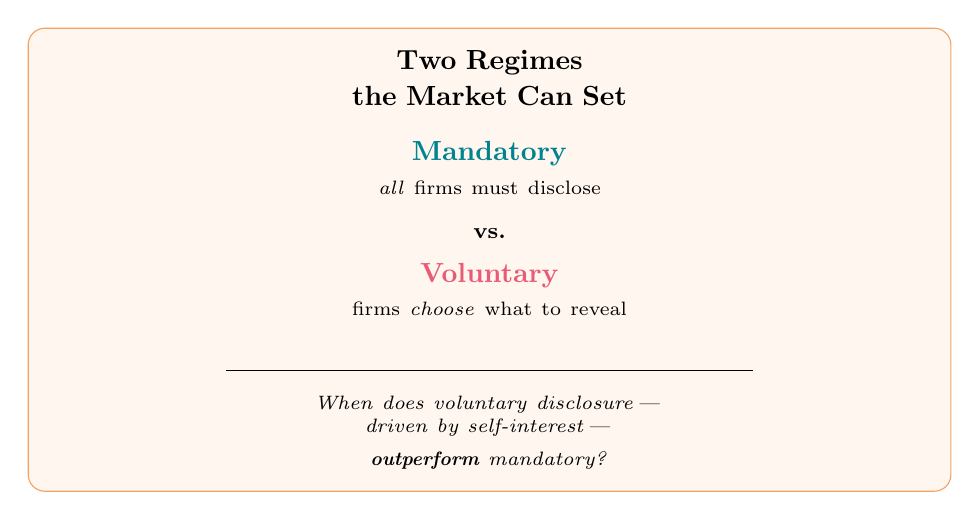
\begin{tikzpicture}
          \node[draw=accentGold, fill=accentGold!10, rounded corners=6pt,
                inner sep=8pt, text width=0.92\linewidth, align=center]{
            {\textbf{Two Regimes}}\\[1pt]
            {\textbf{the Market Can Set}}\\[8pt]
            \textcolor{primaryTeal}{\textbf{Mandatory}}\\
            {\scriptsize \textit{all} firms must disclose}\\[4pt]
            {\footnotesize\textbf{vs.}}\\[4pt]
            \textcolor{accentCoral}{\textbf{Voluntary}}\\
            {\scriptsize firms \textit{choose} what to reveal}\\[8pt]
            \rule{0.6\linewidth}{0.4pt}\\[6pt]
            {\scriptsize\textit{When does voluntary disclosure\,---\,\\driven by self-interest\,---\,\\
            \textbf{outperform} mandatory?}}
          };
        \end{tikzpicture}
      \end{center}
    \end{column}

  \end{columns}
\end{frame}

% ======================================================================
\section{Problem Formulation}
% ======================================================================

\begin{frame}{Game-Theoretic Model}
  \begin{center}
  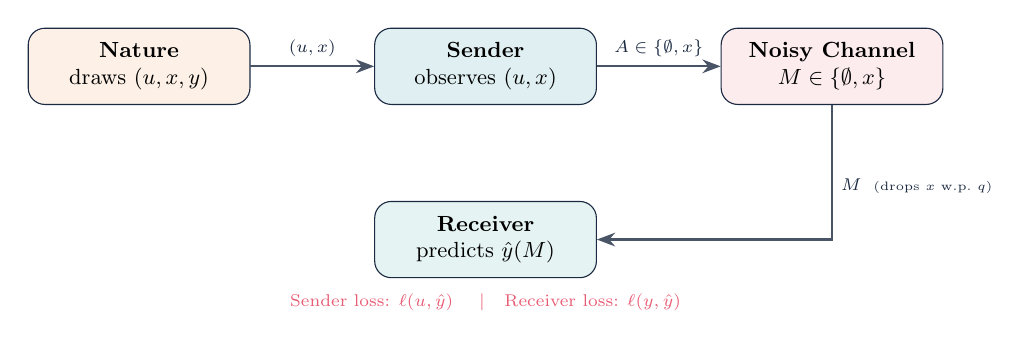
\begin{tikzpicture}[
    scale=0.88, transform shape,
    stage/.style={rectangle, draw=primaryDark, fill=primaryDark!6, rounded corners=6pt,
                  minimum width=3.2cm, minimum height=1.1cm, align=center, font=\small},
    arrow/.style={-Stealth, thick, primaryDark!80},
    label/.style={font=\scriptsize, primaryDark}
  ]
    \node[stage, fill=accentGold!15] (nature) at (0,0) {\textbf{Nature}\\draws $(u, x, y)$};
    \node[stage, fill=primaryTeal!12] (sender) at (5,0) {\textbf{Sender}\\observes $(u, x)$};
    \node[stage, fill=accentCoral!12] (channel) at (10, 0) {\textbf{Noisy Channel}\\$M \in \{\emptyset, x\}$};
    \node[stage, fill=successGreen!12] (receiver) at (5, -2.5) {\textbf{Receiver}\\predicts $\hat{y}(M)$};
    \draw[arrow] (nature) -- node[above, label] {$(u,x)$} (sender);
    \draw[arrow] (sender) -- node[above, label] {$A \in \{\emptyset, x\}$} (channel);
    \draw[arrow] (channel) |- node[right, label, pos=0.3] {$M$\; {\tiny (drops $x$ w.p.\ $q$)}} (receiver);
    \node[below=3pt of receiver, font=\scriptsize, text=accentCoral] {Sender loss: $\ell(u, \hat{y})$ \quad\textbar\quad Receiver loss: $\ell(y, \hat{y})$};
  \end{tikzpicture}
  \end{center}
  \vspace{4pt}
  \begin{columns}[T]
    \begin{column}{0.48\textwidth}
      \begin{block}{Sender Strategy}
        $\cS = \{ A : \cY \times \cX \mapsto \{\emptyset, x\} \}$\\[2pt]
        {\small Disclose full features $x$ or withhold $\emptyset$}
      \end{block}
    \end{column}
    \begin{column}{0.48\textwidth}
      \begin{block}{Receiver Strategy}
        $\cR = \{ \hat{y} : \{\emptyset, \cX\} \mapsto \cY \}$\\[2pt]
        {\small Predict based on received message $M$}
      \end{block}
    \end{column}
  \end{columns}
\end{frame}

\begin{frame}{Stackelberg Equilibrium \& Strategic Advantage}
  We model the interaction as a \textbf{screening game} (Stackelberg):
  \vspace{4pt}
  \begin{enumerate}
    \item \textcolor{primaryTeal}{\textbf{Receiver commits}} to a strategy $\hat{y} \in \cR$
    \item \textcolor{accentCoral}{\textbf{Sender best-responds:}} $\displaystyle A(u,x) = \argmin_{a \in \{\emptyset, x\}} \E[\ell(u, \hat{y}(M)) \mid A = a]$
    \item \textcolor{primaryDark}{\textbf{Outcome realized}} and losses incurred
  \end{enumerate}
  \vspace{8pt}
  \begin{columns}[T]
    \begin{column}{0.48\textwidth}
      \begin{alertblock}{Strategic Risk (Voluntary)}
        \vspace{-6pt}
        $$R_S := \min_{\hat{y} \in \cR} \E[\ell(Y, \hat{y}(M))]$$
        \vspace{-10pt}
      \end{alertblock}
    \end{column}
    \begin{column}{0.48\textwidth}
      \begin{block}{Vanilla Risk (Mandatory)}
        \vspace{-6pt}
        $$R_V := \E[\ell(Y, \hat{y}_V(M))]$$
        \vspace{-10pt}
      \end{block}
    \end{column}
  \end{columns}
  \vspace{8pt}
  \begin{exampleblock}{Definition: Strategic Advantage}
    \centering A \textbf{strategic advantage} exists if $R_S < R_V$\quad\textemdash\quad voluntary disclosure \textit{strictly outperforms} mandatory.
  \end{exampleblock}
\end{frame}

% ======================================================================
\section{Regression Results}
% ======================================================================

\begin{frame}{Regression Setup}
  \begin{itemize}
    \item Outcome space: $\cY = \R$, \quad Loss: $\ell(y, \hat{y}) = (y - \hat{y})^2$ \quad (MSE)
    \item All variables $(U, X, Y)$ have \textbf{zero mean}
    \item Linear receiver: $\hat{y}(\emptyset) = 0$, \quad $\hat{y}(x) = b^\top x$
  \end{itemize}
  \vspace{6pt}
  \begin{columns}[T]
    \begin{column}{0.48\textwidth}
      \begin{block}{Vanilla Risk (Mandatory)}
        \vspace{-4pt}
        $$R_V^\star(q) = \Var(Y) - (1{-}q)\Var(b_Y^\top X)$$
        \vspace{-10pt}
        
        {\small where $b_Y = \Var(X)^{-1}\Cov(X,Y)$ \\ is the OLS weight vector.}
      \end{block}
    \end{column}
    \begin{column}{0.48\textwidth}
      \begin{alertblock}{Strategic Risk (Voluntary)}
        \vspace{-4pt}
        $$R_S(b,q) = \Var(Y) - (1{-}q)\E[G \cdot \Ind{F > 0}]$$
        \vspace{-10pt}
      \end{alertblock}
    \end{column}
  \end{columns}
  \vspace{6pt}
  Key scalar fields governing strategic behavior:
  \begin{center}
    \tikz{
      \node[draw=primaryTeal, fill=primaryTeal!6, rounded corners=5pt, inner sep=6pt] {
        \begin{minipage}{0.78\textwidth}
        \centering
        $F(x,u) := (2u - b^\top x)\, b^\top x$ \hfill \textcolor{primaryTeal}{\scriptsize\textbf{Sender's decision rule}}\\[3pt]
        $G(x,y) := (2y - b^\top x)\, b^\top x$ \hfill \textcolor{accentCoral}{\scriptsize\textbf{Receiver's gain function}}
        \end{minipage}
      };
    }
  \end{center}
\end{frame}

\begin{frame}{Sufficiency Condition for Regression}
  \begin{alertblock}{Theorem (Sufficiency)}
    A \textbf{strategic advantage} exists if $\exists\, b \in \R^d$ such that:
    $$\|U{-}Y\|_2 \;<\; \frac{\E\big[|G(X,Y)|\big] - \Var(b_Y^\top X) - \Var((b{-}b_Y)^\top X)}{4\sqrt{\Var(b_Y^\top X)}}$$
  \end{alertblock}
  \vspace{4pt}
  \begin{columns}[T]
    \begin{column}{0.48\textwidth}
      \begin{center}
        \tikz{
          \node[draw=accentCoral, fill=accentCoral!6, rounded corners=4pt, inner sep=8pt, text width=0.92\linewidth, align=center] {
            \textbf{LHS:} $\|U - Y\|_2$\\[4pt]
            {\small Measures \textit{preference misalignment}\\between sender's preferred\\value $U$ and truth $Y$}
          };
        }
      \end{center}
    \end{column}
    \begin{column}{0.48\textwidth}
      \begin{center}
        \tikz{
          \node[draw=primaryTeal, fill=primaryTeal!6, rounded corners=4pt, inner sep=8pt, text width=0.92\linewidth, align=center] {
            \textbf{RHS:} Feature informativeness\\[4pt]
            {\small Driven by $\E[|G|]$, the expected\\ gain from observing features,\\minus sub-optimality penalty}
          };
        }
      \end{center}
    \end{column}
  \end{columns}
  \vspace{6pt}
  \begin{center}
    {\small\textit{Strategic advantage} $\impliedby$ \textbf{preferences are sufficiently aligned} relative to feature informativeness}
  \end{center}
\end{frame}

\begin{frame}{Necessary Condition for Regression}
  \vspace{-2pt}
  \begin{block}{Theorem (Necessity)}
    {\small A \textbf{necessary condition} for a strategic advantage to exist:}
    \vspace{-4pt}
    $$\max_b \Big( \E\big[|G(X,Y)|\big] - \Var(b_Y^\top X) - \Var((b{-}b_Y)^\top X) \Big) > 0$$
  \end{block}
  \vspace{2pt}
  \begin{exampleblock}{Key Remarks}
    \begin{itemize}\setlength{\itemsep}{0pt}
      \item Necessary condition ensures sufficiency bound is \textbf{non-vacuous}
      \item[\textcolor{accentCoral}{$\star$}] \textbf{Both conditions are independent of channel noise $q$!}\\
            {\small $q$ controls the \textit{magnitude} of the advantage, not its \textit{direction}.}
      \item If conditions hold at $b = b_Y$, they hold for optimal $b$
    \end{itemize}
  \end{exampleblock}
  \vspace{2pt}
  \begin{center}
    \tikz{
      \node[draw=accentGold, fill=accentGold!10, rounded corners=5pt, inner sep=6pt, text width=0.88\textwidth, align=center] {
        \textbf{Takeaway:} The noise $q$ determines the \textbf{magnitude} but \textbf{not the direction} 
        of the strategic advantage.
      };
    }
  \end{center}
\end{frame}

\begin{frame}{Regression: Numerical Validation}
  \vspace{0.5em}
  \begin{columns}[c]
    \begin{column}{0.50\textwidth}
      \centering
      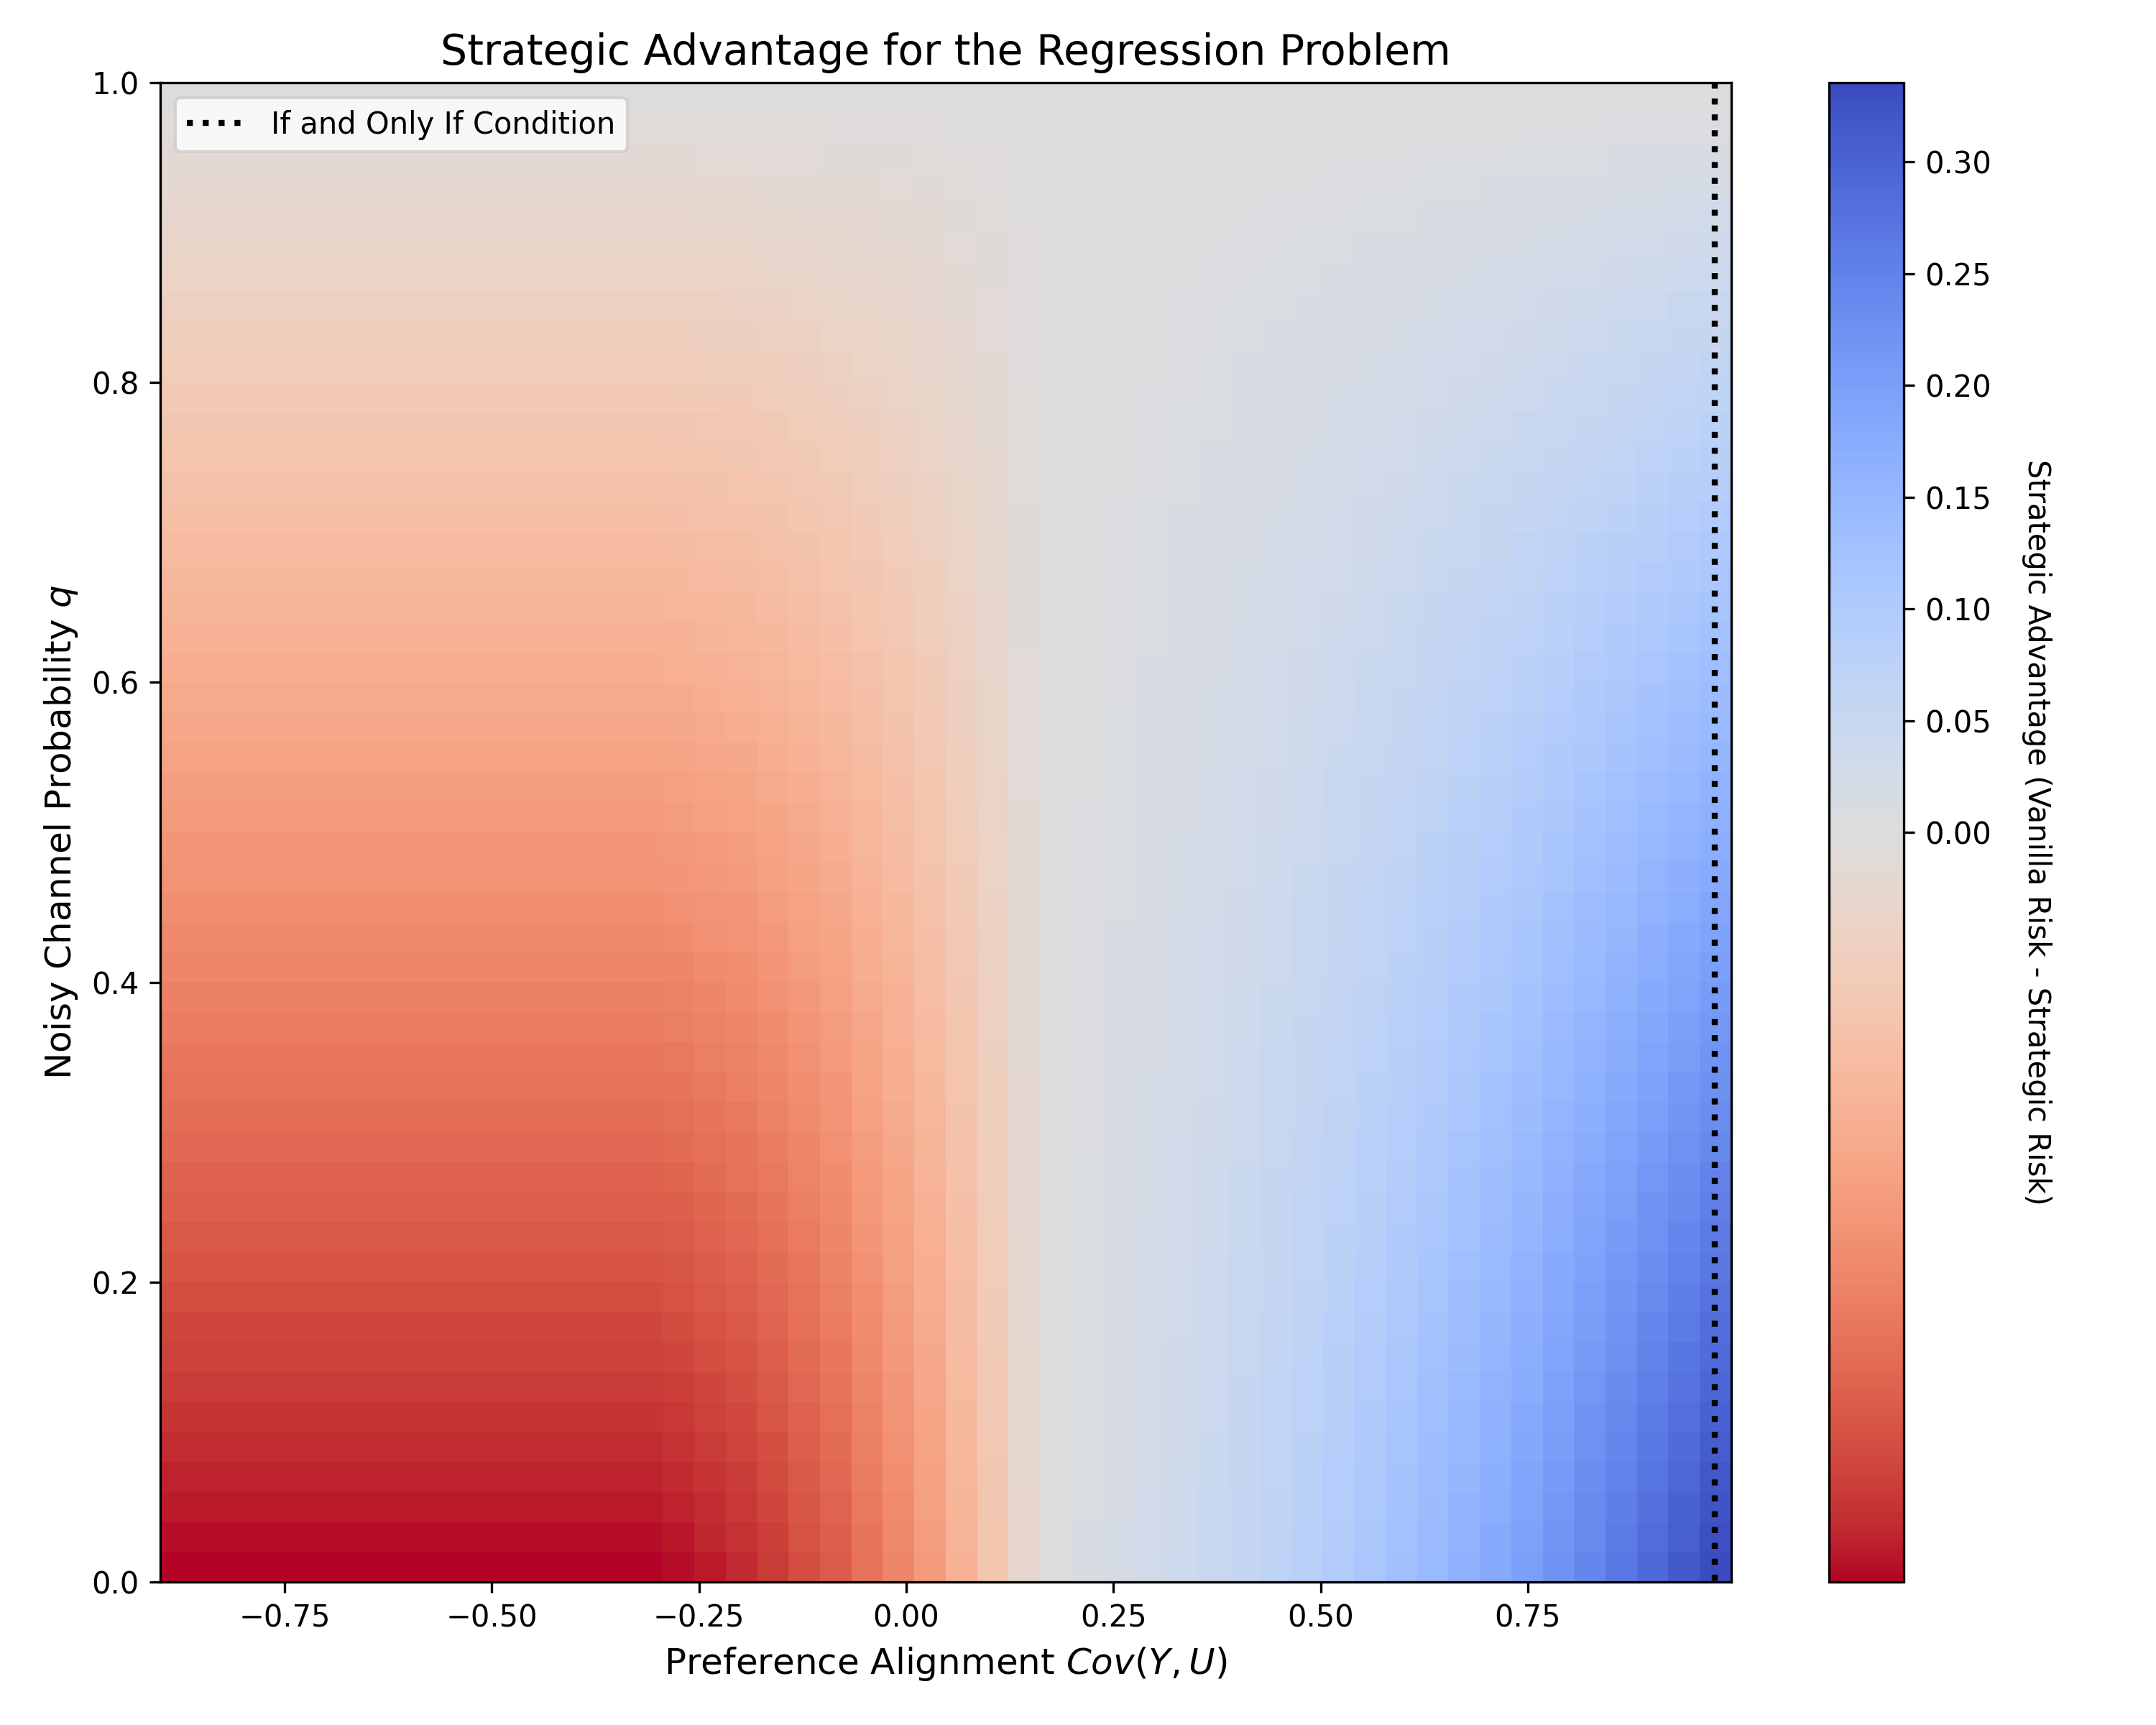
\includegraphics[width=\linewidth]{figures/regression_strategic_advantage.png}
    \end{column}
    \begin{column}{0.47\textwidth}
      \textbf{Setup:}
      \begin{itemize}\setlength{\itemsep}{0pt}
        \item $(X, Y, U) \sim \mathcal{N}(0, \Sigma)$
        \item Unit marginal variances
        \item $\Cov(X,Y) = \Cov(X,U) = 0.2$
      \end{itemize}
      \vspace{2pt}
      \textbf{Parameter sweeps:}
      \begin{itemize}\setlength{\itemsep}{0pt}
        \item $q \in [0, 1]$ {\scriptsize (channel noise)}
        \item $\Cov(Y,U) \in [-1, 1]$  {\scriptsize (preference alignment)}
      \end{itemize}
      \vspace{2pt}
      \begin{exampleblock}{Observation}
        The \textbf{dotted contour} (from our analytical sufficiency bound) reliably delineates the true region of strategic advantage.
      \end{exampleblock}
    \end{column}
  \end{columns}
\end{frame}

% ======================================================================
\section{Classification Results}
% ======================================================================

\begin{frame}{Classification Setup}
  {\small
  \begin{itemize}\setlength{\itemsep}{0pt}
    \item Outcome space: $\cY = \{ \pm 1 \}$, \quad Loss: $\ell(y, \hat{y}) = \Ind{\hat{y} \neq y}$
    \item Preference: $U \in \{ \pm 1 \}$, \quad $\pi_i := \Prob(U = i)$
    \item Assume $\E[Y] > 0$ (label $+1$ is the majority class)
  \end{itemize}
  }
  \vspace{-2pt}
  \begin{columns}[T]
    \begin{column}{0.48\textwidth}
      \begin{block}{Vanilla Risk}
        \vspace{-8pt}
        \begin{align*}
          R_V^\star(q) &= q\,\Prob(Y = -\sgn(\E[Y])) \\
          &\quad + (1{-}q)\,\E\!\left[\frac{1 - |\eta(X)|}{2}\right]
        \end{align*}
        \vspace{-14pt}
        
        {\small where $\eta(x) = \E[Y \mid X\!=\!x]$.}
      \end{block}
    \end{column}
    \begin{column}{0.48\textwidth}
      \begin{alertblock}{Strategic Risk}
        For default option $i \in \{-1,+1\}$:
        \vspace{-8pt}
        \begin{align*}
          R_{\cS_i}^\star(q) &= \pi_i\, \Prob(Y\!=\!{-i} \mid U\!=\!i)\\
          &+ \pi_{-i}\Big[(1{-}q)\E\!\left[\tfrac{1-|\eta_{-i}|}{2}\right]\\
          &\quad + q\,\Prob(Y\!=\!{-i} \mid U\!=\!{-i})\Big]
        \end{align*}
        \vspace{-12pt}
      \end{alertblock}
    \end{column}
  \end{columns}
  \vspace{-2pt}
  \begin{center}
    \tikz{
      \node[draw=primaryTeal, fill=primaryTeal!6, rounded corners=5pt, inner sep=4pt, text width=0.88\textwidth, align=center] {
        {\small Only \textbf{two} possible strategic receiver strategies:
        default to $+1$ ($\cS_1$) or default to $-1$ ($\cS_{-1}$).}\\
        {\scriptsize The optimal strategy depends on distribution structure and channel noise $q$.}
      };
    }
  \end{center}
\end{frame}

\begin{frame}{Classification: Stackelberg Equilibrium}
  \begin{block}{Theorem (\textbf{Exact Characterization} of Strategic Advantage)}
    Assume $\E[Y] > 0$. We provide an \textbf{if and only if} exact condition for strategic advantage. At max noise ($q=1$), strategy $\cS_1$ is always better. Two scenarios arise:
  \end{block}
  \vspace{1pt}
  \begin{columns}[T]
    \begin{column}{0.48\textwidth}
      \begin{exampleblock}{\centering Case 1: $\cS_1$ dominates $\forall q$}
        {\small When $R_{\cS_1}^\star(0) \le R_{\cS_{-1}}^\star(0)$:}
        \vspace{-6pt}
        \begin{align*}
          &(1{-}q)\biggl[\E\!\left[\tfrac{1-|\eta|}{2}\right]\\
          &\quad - \pi_{-1}\E\!\left[\tfrac{1-|\eta_{-1}|}{2}\right]\\
          &\quad - \pi_1\Prob(Y\!=\!{-1} \mid U\!=\!1)\biggr] > 0
        \end{align*}
        \vspace{-10pt}
        
        {\scriptsize \textcolor{successGreen}{\textbf{Independent of $q$!}} Analogous to regression.}
      \end{exampleblock}
    \end{column}
    \begin{column}{0.48\textwidth}
      \begin{alertblock}{\centering Case 2: Strategy switch at $q^\star$}
        {\small $\exists\, q^\star \in (0,1)$. For $q \ge q^\star$: use $\cS_1$. \\For $q < q^\star$: use $\cS_{-1}$ with:}
        \vspace{-6pt}
        \begin{align*}
          &(1{-}q)\!\left[\E\!\left[\tfrac{1-|\eta|}{2}\right] - \pi_1\E\!\left[\tfrac{1-|\eta_1|}{2}\right]\right]\\[-2pt]
          &+ q\big[\Prob(Y\!=\!{-1}) - \pi_1\Prob(Y\!=\!1 \mid U\!=\!1)\big]\\[-2pt]
          &> \pi_{-1}\Prob(Y\!=\!1 \mid U\!=\!{-1})
        \end{align*}
        \vspace{-10pt}
        
        {\scriptsize \textcolor{accentCoral}{\textbf{Depends on $q$!}} Noise affects existence.}
      \end{alertblock}
    \end{column}
  \end{columns}
\end{frame}

\begin{frame}{Classification: Numerical Validation}
  \vspace{1em}
  \begin{columns}[c]
    \begin{column}{0.50\textwidth}
      \centering
      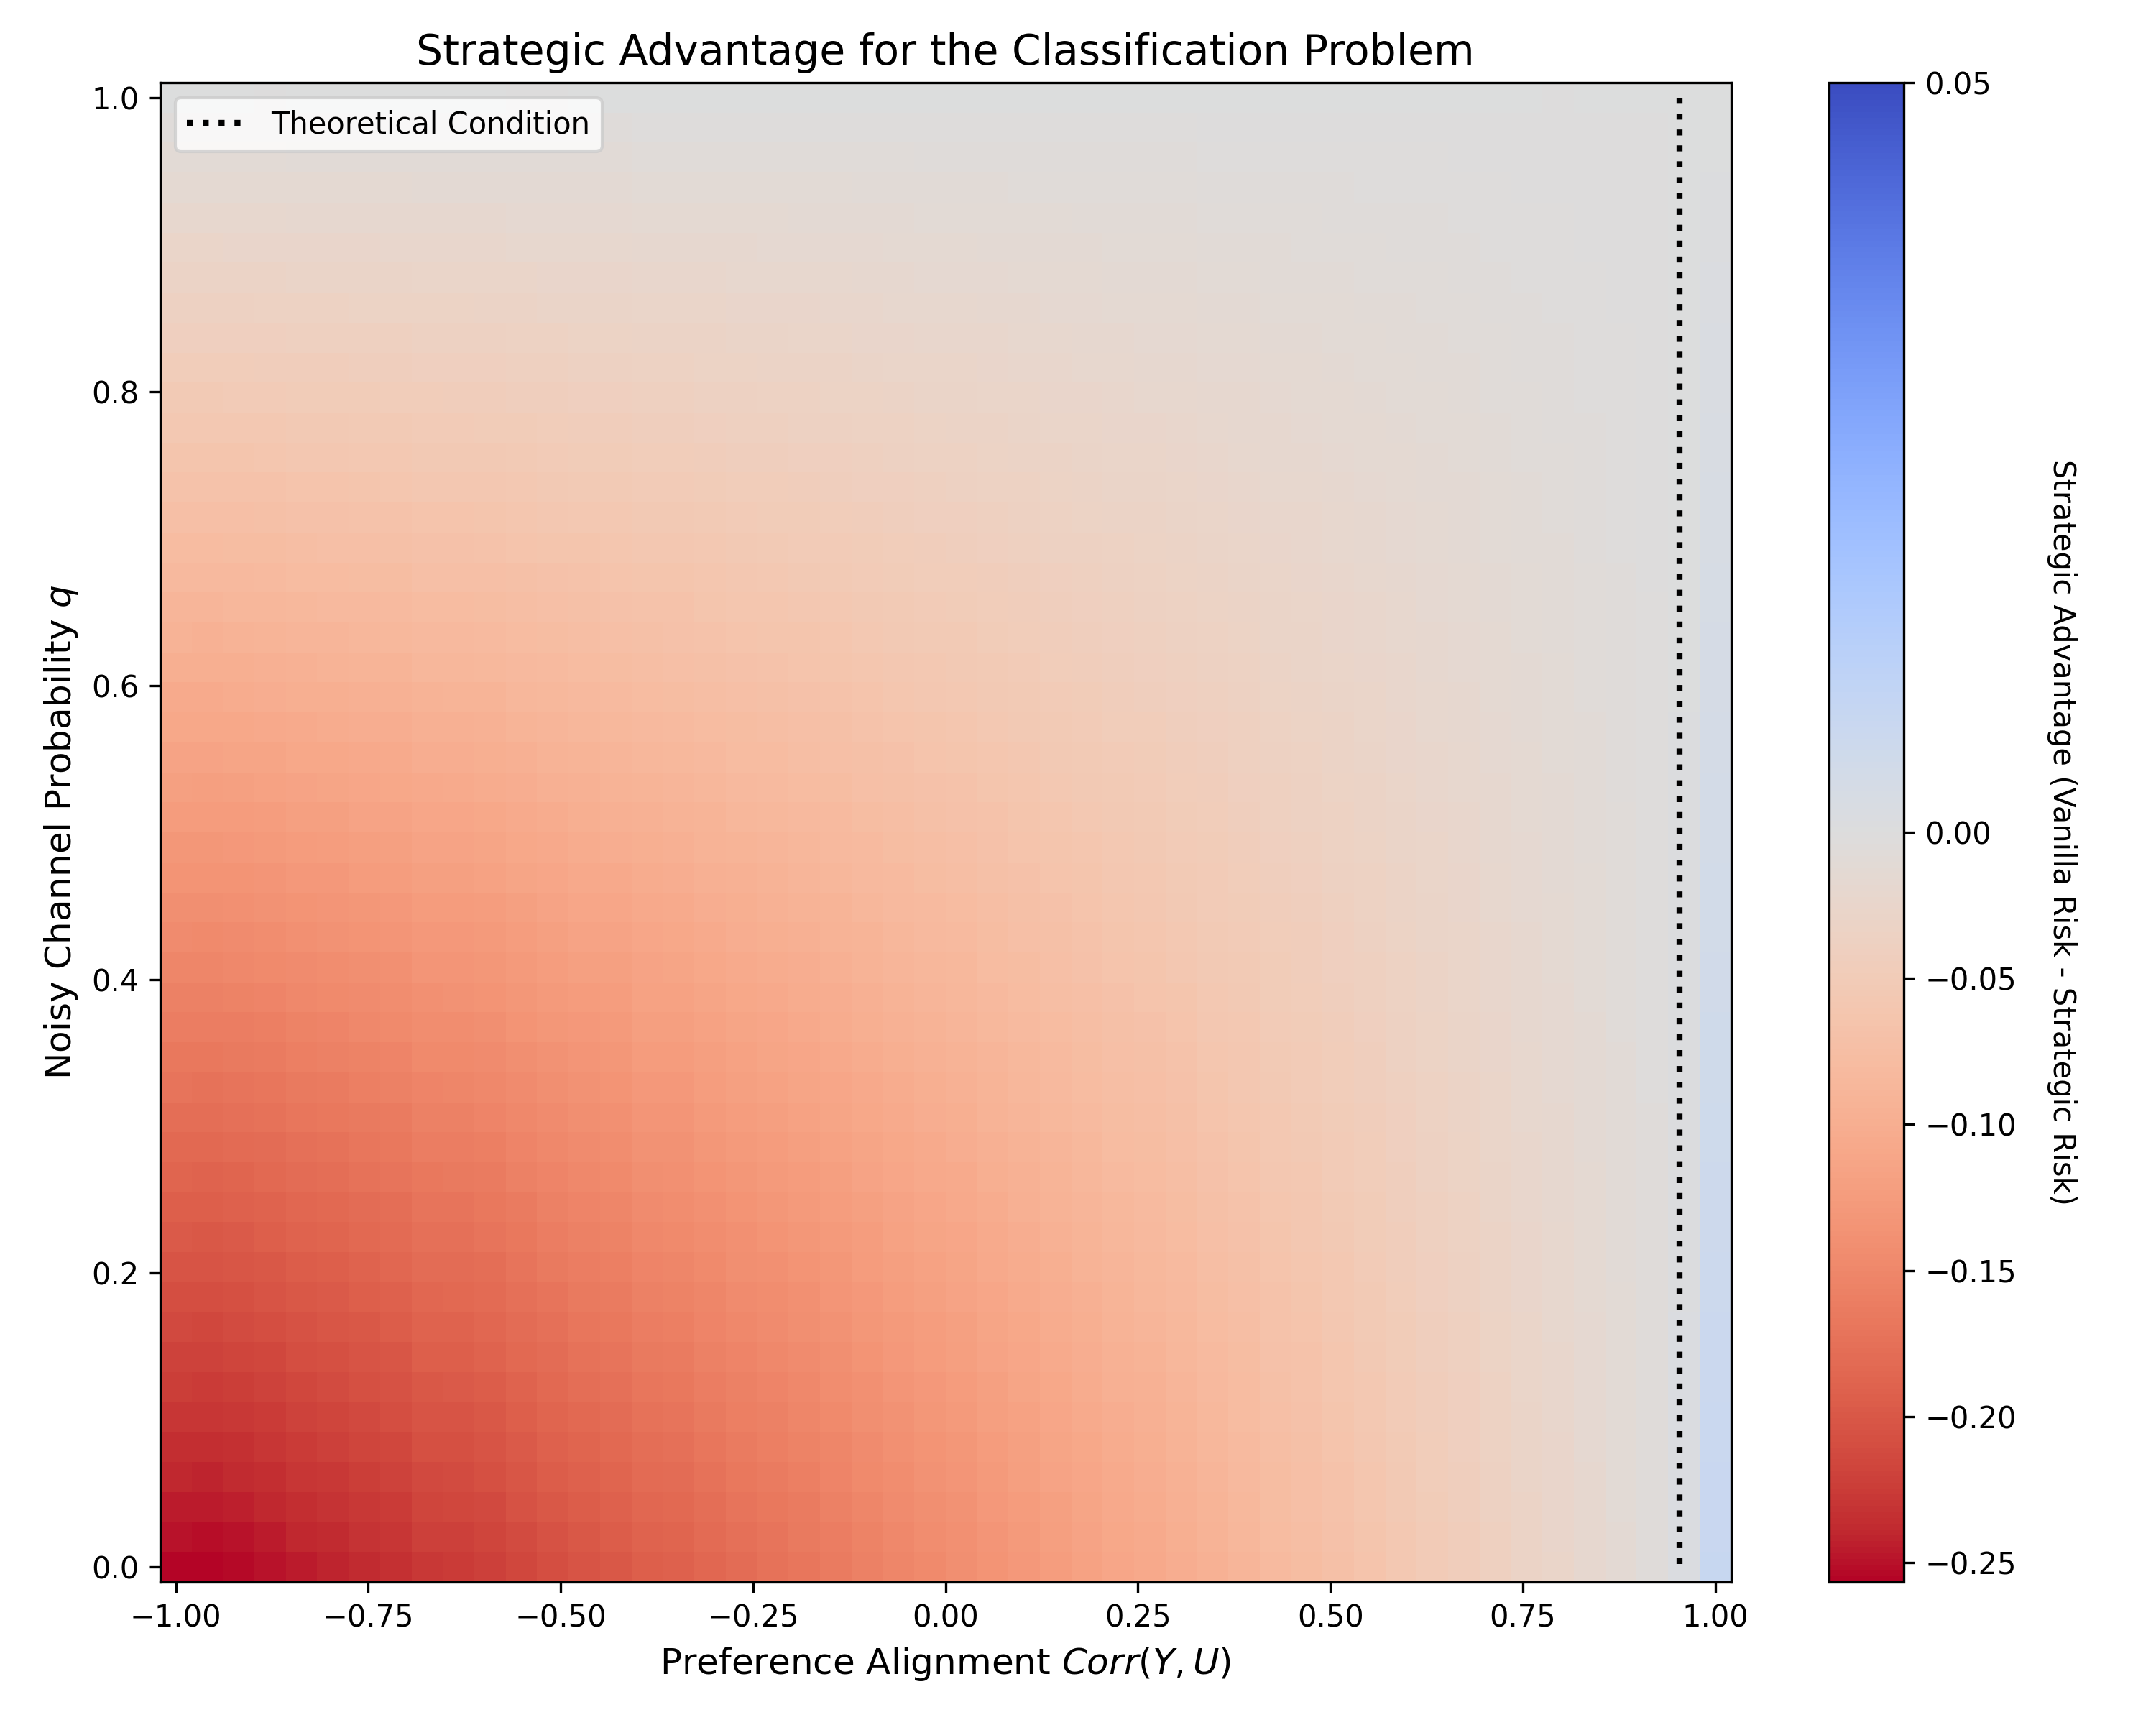
\includegraphics[width=\linewidth]{figures/classification_strategic_advantage.png}
    \end{column}
    \begin{column}{0.47\textwidth}
      \textbf{Setup:}
      \begin{itemize}
        \item $(Y,U) \in \{-1,+1\}^2$
        \item $P(Y\!=\!1) = 0.6$, $P(U\!=\!1) = 0.5$
        \item Features: Gaussian mixture\\
              {\scriptsize $X \mid Y, U \sim Y\mu_Y + U\mu_U + \mathcal{N}(0,1)$}
      \end{itemize}
      \vspace{4pt}
      \textbf{Parameter sweeps:}
      \begin{itemize}
        \item $q \in [0, 1]$ {\scriptsize (channel noise)}
        \item $\Cov(Y,U) \in [-1, 1]$  {\scriptsize (preference alignment)}
      \end{itemize}
      \vspace{4pt}
      \begin{exampleblock}{Validation}
        Analytical boundary matches the empirical advantage region precisely.
      \end{exampleblock}
    \end{column}
  \end{columns}
\end{frame}

% % ======================================================================
% \section{Regression vs.\ Classification: A Comparison}
% % ======================================================================

% \begin{frame}{Decision Problem Comparison}
%   \begin{center}
%   \renewcommand{\arraystretch}{1.3}
%   \begin{tabular}{@{} p{3.2cm} p{5cm} p{5cm} @{}}
%     \toprule
%     & \textcolor{primaryTeal}{\textbf{Regression}} & \textcolor{accentCoral}{\textbf{Classification}} \\
%     \midrule
%     \textbf{Outcome space} & $\cY = \R$ & $\cY = \{-1, +1\}$ \\
%     \textbf{Loss function} & Squared loss $(y - \hat{y})^2$ & 0-1 loss $\Ind{\hat{y} \neq y}$ \\
%     \textbf{Strategies} & Continuous family & Only two: $\cS_1$ or $\cS_{-1}$ \\
%     \textbf{Dep.\ on $q$} & \textcolor{successGreen}{\textbf{Independent}} & \textcolor{accentCoral}{\textbf{Can depend}} (Case 2) \\
%     \textbf{Sufficiency} & Closed-form bound & Case-based equilibrium \\
%     \bottomrule
%   \end{tabular}
%   \end{center}
%   \vspace{4pt}
%   \begin{center}
%     \tikz{
%       \node[draw=deepPurple, fill=deepPurple!6, rounded corners=6pt, inner sep=8pt, text width=0.88\textwidth, align=center] {
%         \textbf{Common thread:} In both settings, the degree of \textit{preference alignment}\\
%         between sender ($U$) and ground truth ($Y$) is the critical structural determinant.
%       };
%     }
%   \end{center}
% \end{frame}

% ======================================================================
\section{Conclusion}
% ======================================================================

\begin{frame}{Summary of Contributions}
  \begin{center}
  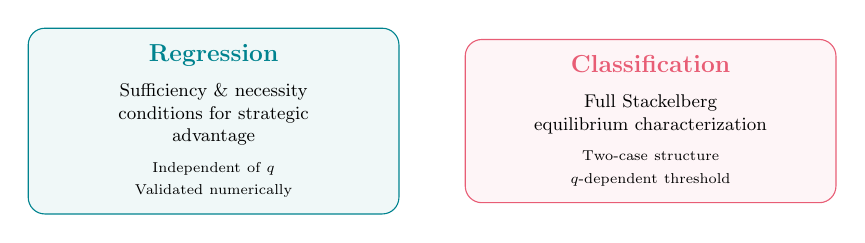
\begin{tikzpicture}[
    scale=0.74, transform shape,
    card/.style={rectangle, rounded corners=6pt,
                 minimum width=6.2cm, minimum height=2.4cm, align=center, 
                 text width=5.8cm, font=\small, inner sep=8pt}
  ]
    \node[card, draw=primaryTeal, fill=primaryTeal!6] (r) at (0, 0) {
      {\large\textbf{\textcolor{primaryTeal}{Regression}}}\\[6pt]
      Sufficiency \& necessity\\conditions for strategic\\advantage\\[4pt]
      {\scriptsize Independent of $q$}\\
      {\scriptsize Validated numerically}
    };
    \node[card, draw=accentCoral, fill=accentCoral!6] (c) at (7.5, 0) {
      {\large\textbf{\textcolor{accentCoral}{Classification}}}\\[6pt]
      Full Stackelberg\\equilibrium characterization\\[4pt]
      {\scriptsize Two-case structure}\\
      {\scriptsize $q$-dependent threshold}
    };
  \end{tikzpicture}
  \end{center}
  \vspace{0pt}
  \begin{center}
    \tikz{
      \node[draw=accentGold, fill=accentGold!10, rounded corners=6pt, inner sep=6pt, text width=0.94\textwidth, align=center] {
        \textbf{Key Drivers of Strategic Advantage}\\[1pt]
        {\small \textcolor{primaryTeal}{\textbf{Regression:}} driven by \textbf{$U, Y$ alignment.}
        (Favourable when preferences align with ground truth.)}\\[3pt]
        {\small \textcolor{accentCoral}{\textbf{Classification:}} driven by the competition between $\mathbb{E}[Y \mid X]$ and the pair ${\mathbb{E}[Y \mid X,U], \mathbb{E}[Y]}$.}
      };
    }
  \end{center}
\end{frame}

\begin{frame}{Limitations \& Future Directions}
  \begin{columns}[T]
    \begin{column}{0.48\textwidth}
      \begin{alertblock}{\centering Limitations}
        \begin{itemize}
          \item Sufficiency bounds can be \textbf{conservative} for some distribution families
          \item Restricted to \textbf{linear} receiver strategies in regression
          \item Classification analysis limited to \textbf{binary} labels
          \item Environment (joint distribution) assumed \textbf{known}
        \end{itemize}
      \end{alertblock}
    \end{column}
    \begin{column}{0.48\textwidth}
      \begin{exampleblock}{\centering Future Directions}
        \begin{itemize}
          \item \textbf{Unknown environment:} online learning when receiver must learn the distribution
          \item \textbf{Non-linear predictors:} kernels, neural networks
          \item \textbf{Multi-sender} competitive environments
          \item \textbf{Partial disclosure:} reveal subsets of features
          \item \textbf{Tighter bounds:} closing the sufficiency--necessity gap
        \end{itemize}
      \end{exampleblock}
    \end{column}
  \end{columns}
\end{frame}

% ======================= THANK YOU =======================
{
\setbeamercolor{background canvas}{bg=primaryDark}
\begin{frame}[plain, noframenumbering]
  \vfill
  \begin{center}
    {\Huge\color{white}\textbf{Thank You!}}\\[20pt]
    {\Large\color{accentCoral}Questions \& Discussion}\\[24pt]
    \tikz{
      \node[draw=accentGold, fill=accentGold!12, rounded corners=6pt, inner sep=12pt, text width=0.85\textwidth, align=center] {
        \color{primaryDark}\textbf{Key Message}\\[4pt]
        \color{primaryDark}\textit{Voluntary disclosure can outperform mandatory disclosure}\\
        \color{primaryDark}\textit{when participant preferences are \textbf{sufficiently aligned} with ground truth.}
      };
    }
  \end{center}
  \vfill
\end{frame}
}

\end{document}
